% Created 2018-04-17 Tue 12:11
% Intended LaTeX compiler: pdflatex
\documentclass[11pt]{article}
\usepackage[utf8]{inputenc}
\usepackage[T1]{fontenc}
\usepackage{graphicx}
\usepackage{grffile}
\usepackage{longtable}
\usepackage{wrapfig}
\usepackage{rotating}
\usepackage[normalem]{ulem}
\usepackage{amsmath}
\usepackage{textcomp}
\usepackage{amssymb}
\usepackage{capt-of}
\usepackage{hyperref}
\usepackage{listings}
\date{\today}
\title{Urschleim in Silicon: The Slideshow}
\hypersetup{
 pdfauthor={},
 pdftitle={Urschleim in Silicon: The Slideshow},
 pdfkeywords={},
 pdfsubject={},
 pdfcreator={Emacs 25.3.1 (Org mode 9.1.6)}, 
 pdflang={English}}
\begin{document}

\maketitle
\setcounter{tocdepth}{1}
\tableofcontents


\section*{Introductory Remarks}
\label{sec:org676fa7a}
\section*{The Concept of Return-Oriented Programming}
\label{sec:org3d7dd21}
\subsection*{The Fundamental Problem of Cybersecurity}
\label{sec:org2204cb8}
At bottom, there is no essential distinction between data and code.

"Data" is just information your system trusts. 
\subsection*{Consider the Stack}
\label{sec:org41207fe}
\begin{center}
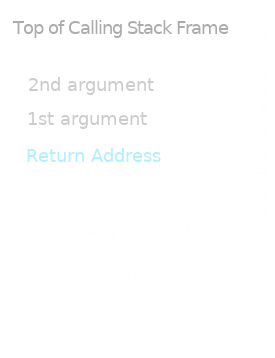
\includegraphics[width=.9\linewidth]{../images/stack_frame.png}
\end{center}
\begin{itemize}
\item the hacker feeds some input data to the process
\item which is written to a buffer in stack memory
\item but which overruns the buffer
\item corrupting the frame's return address
\end{itemize}

\subsection*{Consider the Stack, Smashed}
\label{sec:orgfb842f7}

\begin{center}
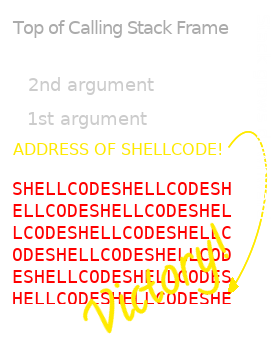
\includegraphics[width=.9\linewidth]{../images/stack_frame_attack.png}
\end{center}
\begin{itemize}
\item so that it points into the buffer
\item a buffer that turns out to contain machine code
\item to which the program counter "returns"
\item executing it just as it would its own instructions!
\end{itemize}

\subsection*{\(\textit{DEP}~~/~~W \oplus X\)}
\label{sec:orgcbe1102}
\begin{center}
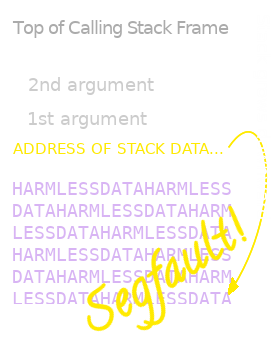
\includegraphics[width=.9\linewidth]{../images/stack_frame_attack_w^x.png}
\end{center}
\begin{itemize}
\item One way of mitigating this is to try to ensure that no page of memory is both writeable \textbf{and} executable.
\item The idea being that \emph{data} should be writeable, but never executable, while \emph{code} should be executed, but not written at runtime.
\end{itemize}



\subsection*{So, is code "wherever the program counter's pointing"?}
\label{sec:org7572833}
\subsection*{No. It's far worse than that.}
\label{sec:org35f607f}
\subsection*{Subverting \(~~W\oplus X\)}
\label{sec:orge062217}
\begin{itemize}
\item \(W\oplus X\) may prevent the \emph{execution} of input data, but it doesn't prevent attempts to \emph{return} to that data.
\item Why should the hacker need to supply their own machine code?
\item There's quite a bit just laying around, in executable memory.
\item Why not just build a payload with whatever's handy?
\end{itemize}
\subsection*{It's what MacGyver would do}
\label{sec:org049a52b}
But how?
\subsection*{\(W\oplus X~~\) is a Leaky Abstraction}
\label{sec:orgdb7034d}
\begin{itemize}
\item It rests on all-too-narrow concepts of "instruction" and "execution".
\item The payload's \emph{instructions} don't need to be bytes of machine code.
\item They just need to influence control flow, in a controllable way.
\end{itemize}
\subsection*{So is the \emph{Structured Programming Machine Model}}
\label{sec:orgda05ca4}
\begin{itemize}
\item The machine model on which structured programming is based already carves up an executable into chunks that \textbf{return} control after being dispatched.
\item To the programmer, these are "functions", but this is too granular a viewpoint.
\item \emph{Any} chunk of code ending with a \textbf{return} returns control to whomever controls the stack.
\item And our data controls the stack!
\end{itemize}

\subsection*{The ROVM supervenes on the SPMM}
\label{sec:orgbfd030e}
\begin{center}
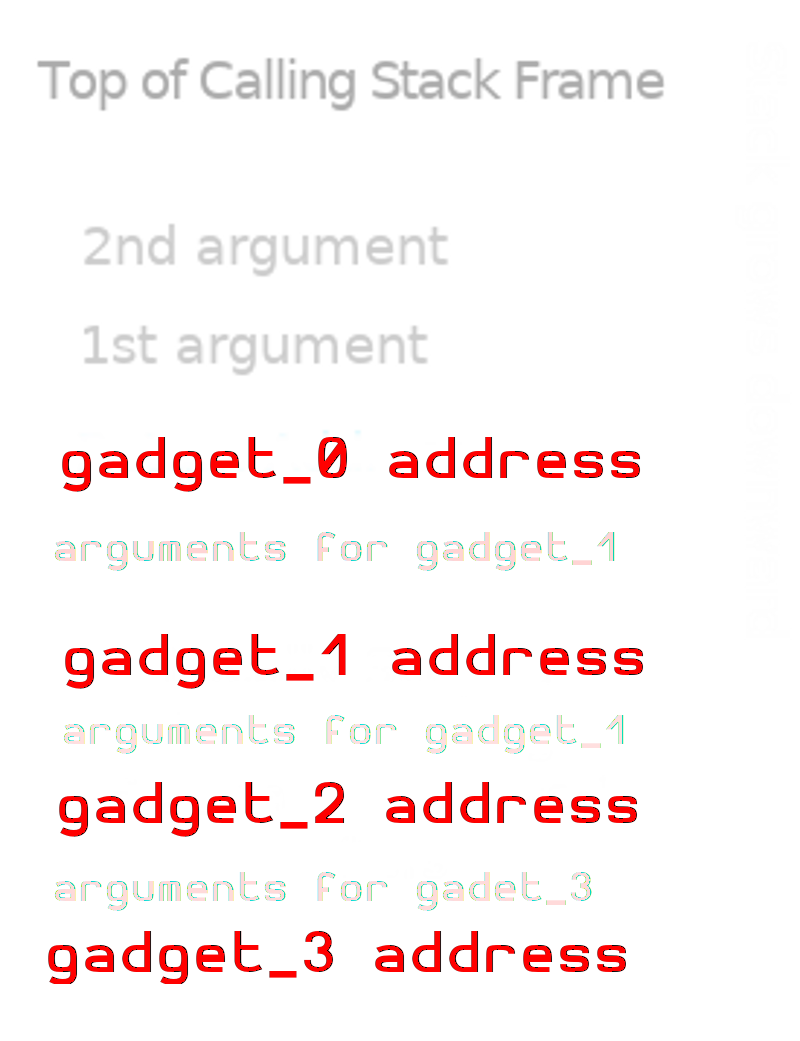
\includegraphics[width=.9\linewidth]{../images/stack_frame_rop.png}
\end{center}
\begin{itemize}
\item Chunks of code that return control are called "gadgets".
\item They form a spontaneous ISA, whose \textbf{program counter} is the \textbf{stack pointer} of the underlying architecture.
\item Let's call this ISA a "Return-Oriented Virtual Machine".
\end{itemize}

\subsection*{We can program this machine with input data\ldots{}}
\label{sec:org4830365}
\begin{itemize}
\item All we need to do is to discover and supply a buffer of instructions.
\item These are not instructions for the underlying architecture, but for the ROVM.
\item \(W\oplus X\) is blissfully unaware of the ROVM, and powerless to prevent us from executing data as \emph{ROVM} code.
\end{itemize}

\subsection*{\ldots{}and so can natural selection.}
\label{sec:orge4173d8}

\section*{Design and Implementation of ROPER}
\label{sec:org902e5c6}

\subsection*{Bird's eye view}
\label{sec:org47b09b6}
\begin{center}
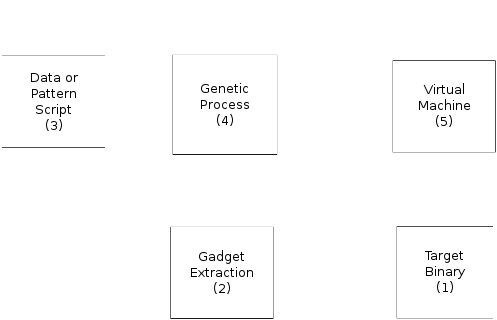
\includegraphics[width=.9\linewidth]{../images/birdseye_white.png}
\end{center}

\subsection*{Gadget Harvest}
\label{sec:orge0375ee}
\begin{center}
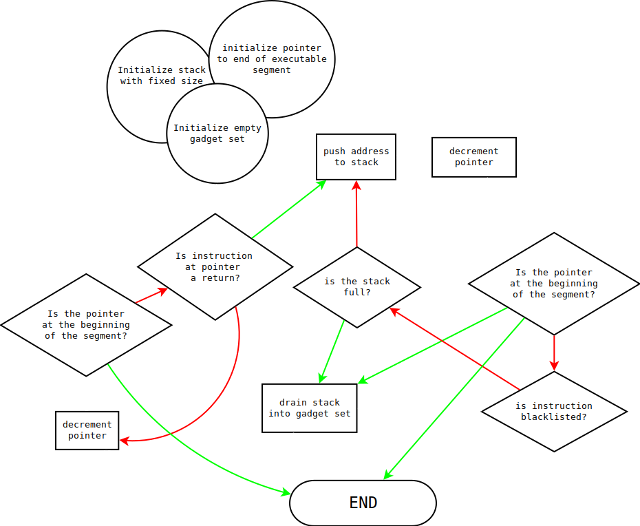
\includegraphics[width=.9\linewidth]{../images/gadget-harvest.png}
\end{center}

\subsection*{Tournament Selection}
\label{sec:orgd197e29}
\begin{center}
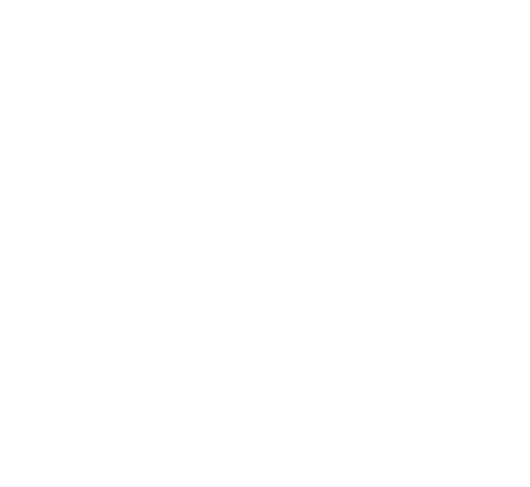
\includegraphics[width=.9\linewidth]{../images/tournament.png}
\end{center}

\subsection*{Genomic Structure}
\label{sec:orgd176949}
\begin{itemize}
\item Each genome is a one-dimensional \emph{chain} composed of \emph{clumps}.
\item A \emph{clump} is a gadget address \(a\), followed by \(\texttt{SP}_\Delta(a)-1\) machine words
\item where \(\texttt{SP}_\Delta(a)\) is the (estimated) number of words that \(*a\) will pop from the stack, when run.
\item Several "epigenetic" fields of metadata are also associated with both the \emph{chain} and \emph{clump} structures.
\end{itemize}

\subsection*{Genetic Operators: Clumpwise Mutation}
\label{sec:org9c68dee}
\begin{itemize}
\item address substitution
\item arithmetical \& logical manipulation of dwords
\item indirection/dereference of dwords
\item permutation of pairs of dwords
\end{itemize}

\subsection*{Genetic Operators: Chainwise Crossover}
\label{sec:orgb7bf510}
\begin{itemize}
\item restricted to single-point crossover
\item splice point selected by weighted random choice, using the average of each link's previous hosts' fitness scores, to favour adaptive gene linkage
\item recently, a mechanism to promote homologous crossover in fitter specimens has been introduced
\end{itemize}

\subsection*{Algebraic properties of genetic operators}
\label{sec:org2872d90}
\begin{itemize}
\item Mutations form a cyclic group under concatenation.
\item Crossover is associative, forms a cyclic group under concatenation, and commutes with mutation.
\item These properties permit the operators to traverse the space of genetic combinations without ratcheting the population into a corner.
\end{itemize}

\subsection*{Ontogenesis}
\label{sec:orgecd27af}
\begin{itemize}
\item The genotype is mapped to its phenotype by executing it in an emulated CPU, into which the binary from which it was derived has been loaded.
\item The chain is serialized into an array of dwords,
\item loaded into the stack space of the target process
\item its initial address is popped into the CPU's program counter
\item and the emulation begins.
\end{itemize}

\subsection*{Ontogenesis}
\label{sec:orgdabd3a3}
\begin{itemize}
\item This process returns a snapshot of CPU behaviour from the chain's execution:
\end{itemize}
\begin{itemize}
\item the resulting register values
\item a window of memory surrounding each dereferenced register value
\item and the list of addresses visited by the chain.
\item This data is passed to one of several task-specific fitness functions.
\end{itemize}

\subsection*{Evaluation Process}
\label{sec:org2c2eb9a}
\begin{center}
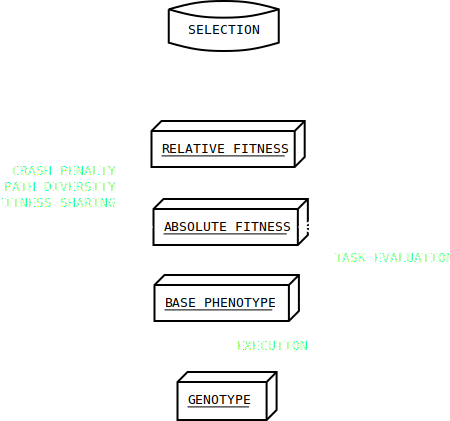
\includegraphics[width=.9\linewidth]{../images/evaluation_model_white.png}
\end{center}


\section*{Experimental Studies}
\label{sec:org0f659e5}

\subsection*{The Environment}
\label{sec:orgca90f92}
\begin{center}
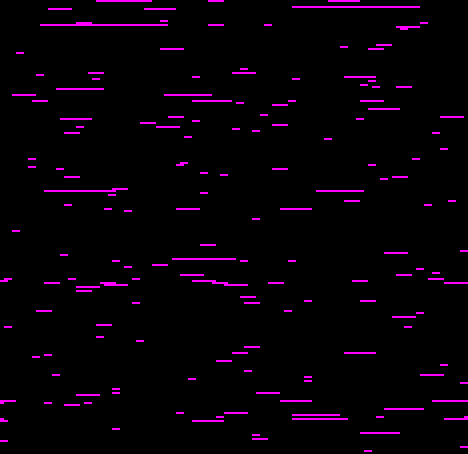
\includegraphics[width=.9\linewidth]{../../thesis/images/tomato-RT-N18U-httpd_heatmap.png}
\end{center}

Distribution of gadgets in \texttt{tomato-RT-N18U-httpd}.


\subsection*{Tasks and Fitness Functions}
\label{sec:orge6232b0}
\begin{itemize}
\item An arbitrary and inscrutable fitness function
\item System call preparation
\item Classification tasks:
\begin{itemize}
\item An artificial, linearly-separable dataset
\item The Iris dataset
\end{itemize}
\item A Snake game
\end{itemize}



\subsubsection*{Kafka function with Crash Penalty}
\label{sec:orgbdd19c1}

The address visitation heatmap shows no evident loss of diversity,
even after 212 seasons, suggesting a robustly ergodic system. 
\begin{center}
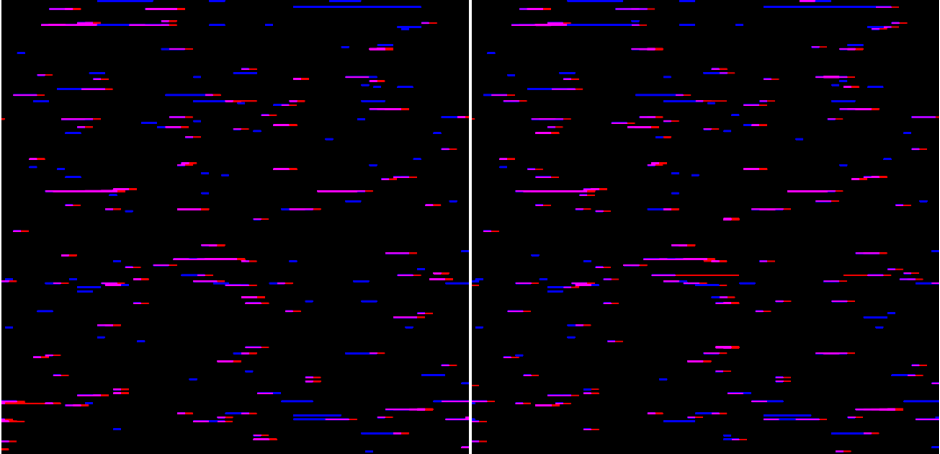
\includegraphics[width=.9\linewidth]{../../thesis/images/plots/xeqcyv_kafka_heatmap_beginning_end.png}
\end{center}

\subsubsection*{System Call Preparation}
\label{sec:org77df97e}

\begin{itemize}
\item The goal here is to prepare the CPU for a system call, with the registers containing and pointing to the necessary arguments.
\item The fitness function uses a combination of numerical distance and bitwise hamming distance, for immediate values, and memory proximity for indirect values.
\item A successful evolutionary run delivers a payload that can be used for practical purposes.
\end{itemize}


\subsubsection*{System Call Preparation}
\label{sec:orgc50dfda}

Champion of the \emph{Wiwzuh} population:
\lstset{language=asm,label= ,caption= ,captionpos=b,numbers=none}
\begin{lstlisting}
  0000b4ac        pop {r4, r5, r6, r7, r8, pc}

  0000d1a0        cmp r0, #0
  0000d1a4        popeq {r3, r4, r5, pc}

  00016654        cmp r0, #0
  00016658        ldr r3, [pc, #4]
  0001665c        moveq r0, r3
  00016660        pop {r3, pc}

  0001706c        ldm sp, {r0, r1}
  00017070        add sp, sp, #0x10
  00017074        pop {r4, r5, r6, pc}

;; R0:  0001f62f   R2:  00000000
;; R1: &0001f62f   R7:  0000000b

;; to call execv("/tmp/flashXXXXXX", ["/tmp/flashXXXXXX"], NULL) 
  00018fc4        svcvc #0xffffff
\end{lstlisting}

\subsubsection*{Fitness landscape traversed by the \emph{wiwzuh} population}
\label{sec:orgb851e23}
\begin{center}
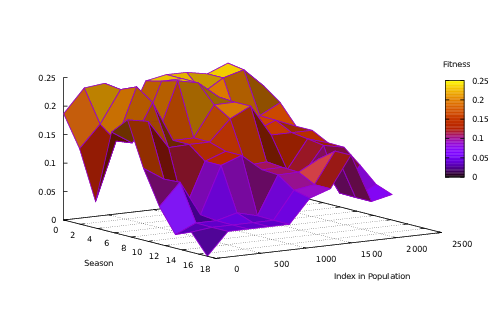
\includegraphics[width=.9\linewidth]{../../thesis/images/plots/wiwzuh_syscall_gaussian_3.png}
\end{center}

\subsubsection*{The Enigma of Stray Gadgets}
\label{sec:org406b458}
\begin{itemize}
\item This task also produced a number of specimens whose traces are too long and complex to display in detail here, but which were especially interesting for their labyrinthine nature, and the degree to which their execution traces strayed from the harvested gadget set.
\item I will nevertheless \textbf{try} to display one here.
\end{itemize}

\subsubsection*{}
\label{sec:orgb879aa5}
\subsubsection*{The Enigma of Stray Gadgets}
\label{sec:orgebdda3b}
These were of interest in two respects:

\begin{itemize}
\item they contained complex \emph{heuristic breakers} making them likely to bypass various IDS systems in the literature, as a sheer evolutionary \emph{spandrel}
\item theoretically, their behaviour was enigmatic. Straying is dangerous for chains, and comes with great risk of crashing, yet it appeared with \emph{prima facie} improbable frequency in our populations.
\end{itemize}


\subsubsection*{A simple classification task}
\label{sec:orge8c6789}
\begin{itemize}
\item For the classification tasks, I initially used a common, bid-based algorithm to map behaviour to classification decisions on data samples.
\item A set of output registers was mapped to the class list, and data was classified according to the register containing the greatest signed value.
\end{itemize}

\subsubsection*{Fair initial results}
\label{sec:orgc465b14}
\begin{center}
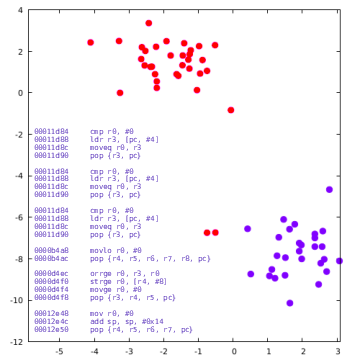
\includegraphics[width=.9\linewidth]{../images/plots/kathot_champion.png}
\end{center}

\subsubsection*{An interesting case of malignancy}
\label{sec:orga32e9d7}

\begin{center}
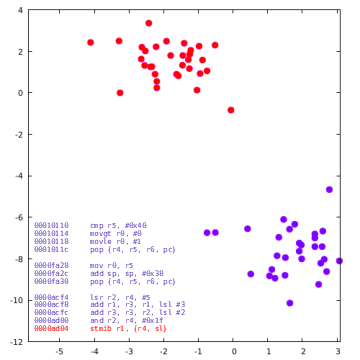
\includegraphics[width=.9\linewidth]{../images/plots/fizwej_perfect_crash.png}
\end{center}

Here, the gene responsible for correct classification of the data was also responsible for crashing the execution. It rapidly took over the population.

\subsubsection*{An interesting case of malignancy}
\label{sec:orgaca287e}
\begin{center}
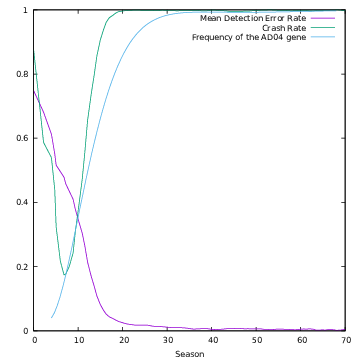
\includegraphics[width=.9\linewidth]{../images/plots/fizwej-badgenes.png}
\end{center}

\subsubsection*{The Iris Dataset}
\label{sec:org9ce225f}
\begin{center}
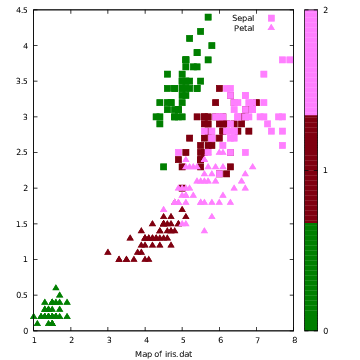
\includegraphics[width=.9\linewidth]{../images/plots/iris_plot.png}
\end{center}

\subsubsection*{ROPER on the Iris Dataset}
\label{sec:orgde4f25c}
\begin{itemize}
\item This dataset proved a serious challenge for ROPER, which rarely achieved better than a 66\% detection rate (using the bid-bin method).
\item Success only came with the introduction of a fitness sharing mechanism.
\end{itemize}

\subsubsection*{Iris without Fitness Sharing}
\label{sec:orgb3881c7}
\begin{center}
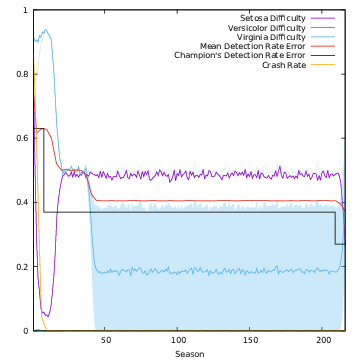
\includegraphics[width=.9\linewidth]{../images/plots/nosharing.png}
\end{center}

\subsubsection*{Iris with Fitness Sharing}
\label{sec:org12798ba}
\begin{center}
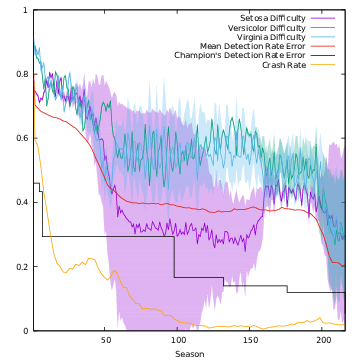
\includegraphics[width=.9\linewidth]{../images/plots/sharing.png}
\end{center}

\subsubsection*{Bit-masks over Bid-bins}
\label{sec:org94c9d7d}

The uneven distribution of register usage puts a skew on any
classification task using the register bid-bin method. 
\begin{center}
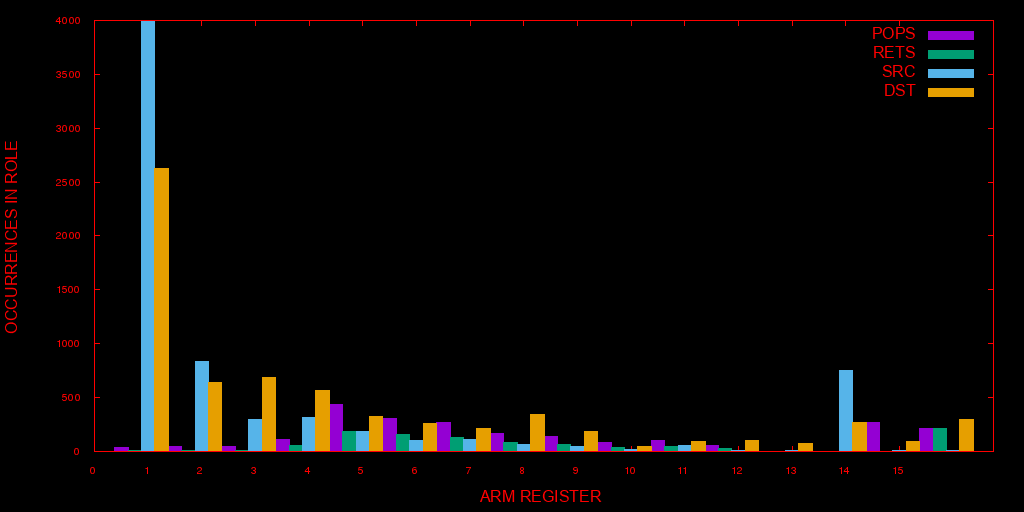
\includegraphics[width=.9\linewidth]{../images/tomato.png}
\end{center}

\subsubsection*{Bitmask Classification Specimens}
\label{sec:orgce98f5d}
\begin{verbatim}
IN:  ffffff98 d
0000b4b4       | pop {r4, r5, r6, r7, r8, pc}
0000d9a8       | cmp r0, #0
0000d9ac       | moveq r0, r3
0000d9b0       | pop {r3, pc}
0001010c       | rsb r5, r5, r0
00010110       | cmp r5, #0x40
00010114       | movgt r0, #0
00010118       | movle r0, #1
0001011c       | pop {r4, r5, r6, pc}
0000cdd0       | subs r4, r0, #0
0000cdd4       | popeq {r4, r5, r6, pc}
0000d9ac       | moveq r0, r3
0000d9b0       | pop {r3, pc}
00016168       | add r0, r4, r0
0001616c       | pop {r3, r4, r5, pc}
0000ad94       | mov r0, r3
0000ad98       | pop {r4, pc}
0001228c       | add sp, sp, #0x364
00012290       | add sp, sp, #0x400
00012294       | pop {r4, r5, r6, r7, r8, sb, sl, fp, pc}
OUT: ea->0 0->68732e00 ffffff98 ea->0 0->68732e00 0->68732e00 0->68732e00 
.... 0->68732e00 0->68732e00 0->68732e00 0->68732e00 0->68732e00 0->68732e00 2b7eb->0 0->68732e00 0->68732e00 
R0 (bin): 00000000000000000000000011101010
CLASS: RED
\end{verbatim}
Greater complexity in control flow, perfect classification results, no crashing.
\begin{verbatim}
IN:  a3 fffffd6f
0000b4b4       | pop {r4, r5, r6, r7, r8, pc}
0000d9a8       | cmp r0, #0
0000d9ac       | moveq r0, r3
0000d9b0       | pop {r3, pc}
0001010c       | rsb r5, r5, r0
00010110       | cmp r5, #0x40
00010114       | movgt r0, #0
00010118       | movle r0, #1
0001011c       | pop {r4, r5, r6, pc}
0000cdd0       | subs r4, r0, #0
0000cdd4       | popeq {r4, r5, r6, pc}
0000cdd8 stray | ldr r1, [pc, #0x1c]
0000cddc stray | mov r2, r4
0000cde0 stray | mov r0, #0
0000cde4 stray | bl #0x59e0
000127c4 stray | push {r1, r2, r3}
000127c8 stray | push {r0, r1, r2, r4, r5, r6, r7, r8, lr}
000127cc stray | mov r6, r0
000127d0 stray | mov r5, #0x400
000127d4 stray | add r7, sp, #0x28
000127d8 stray | ldr r8, [sp, #0x24]
000127dc stray | mov r0, r5
000127e0 stray | bl #4294933396
0000a374 stray | add ip, pc, #0
0000a378 stray | add ip, ip, #0x1e000
0000a37c stray | ldr pc, [ip, #0x5a8]!
0000a138 stray | str lr, [sp, #-4]!
0000a13c stray | ldr lr, [pc, #4]
0000a140 stray | add lr, pc, lr
0000a144 stray | ldr pc, [lr, #8]!
OUT: 400->0 1bc01->7365720a 1->7368732e 96106ace 1->7368732e 400->0 0->68732e00 
.... 2b02b->1 1bc01->7365720a 0->68732e00 0->68732e00 0->68732e00 28924->a138 2afff->127e4 28868->0 0->68732e00 
R0 (bin): 00000000000000000000010000000000
CLASS: BLUE
\end{verbatim}

\subsubsection*{The Snake Game}
\label{sec:org19e58e3}

\section*{Concluding Remarks}
\label{sec:orgb8f9945}
\end{document}